\documentclass[aspectratio=169,xcolor=svgnames]{beamer}
%\documentclass{beamer}
%%%CHOOSE ASPECT RATIO ABOVE%%%

% \usetheme{LU-spfaff}

\usepackage[utf8]{inputenc}
\usepackage[british]{babel}
\usepackage{grffile}
\usepackage{minted}
\usepackage{csquotes}
\usepackage{tikz}
\usepackage{libertine}
\usepackage{fancyvrb}
% \usefonttheme{serif}

\usetikzlibrary{tikzmark}
\usetikzlibrary {arrows.meta}
\usetikzlibrary{positioning}

\setminted[java]{autogobble=true,bgcolor=LightGray,linenos}
\setminted[python]{autogobble=true,bgcolor=LightGray,linenos}

\setmonofont{Fira Code}

\title[]{Bayesian Statistics}

% \titlecolor{LUGreen} % Choose between LUPink, LULBlue, LUIvory, LUGreen
%\titleimage{\includegraphics[scale=.5]{astro.png}}
% \titleimage{\includegraphics[scale=.6]{lumainb.jpg}}
\author{Noric Couderc}
% \subtitle{Subtitles are currently limited to one line}
\date{\today}
\institute{Lund University\\Department of Computer Science}

\AtBeginSection[]{
  \begin{frame}
  \vfill
  \centering
  \begin{beamercolorbox}[sep=8pt,center,shadow=true,rounded=true]{title}
    \usebeamerfont{title}\textbf{\insertsectionhead}\par%
  \end{beamercolorbox}
  \vfill
  \end{frame}
}

\setbeamertemplate{footline}[frame number]

\begin{document}

\maketitle

\begin{frame}{About Me}
  \begin{columns}
    \column{0.5\textwidth}
    My name is Noric

    \begin{itemize}
    \item 5th year PhD student
    \item From: Digne les Bains, France
    \item Topics: Dynamic program analysis, performance engineering
    \item Supervisors: Christoph Reichenbach, Emma Söderberg
    \end{itemize}

    \column{0.5\textwidth}
    \includegraphics[width=\columnwidth]{/home/noric/Pictures/moi.jpg}

  \end{columns}
\end{frame}

\section{Performance Example}

\begin{frame}
  We show an example of two running times, and
  compare their means
\end{frame}

\begin{frame}
  Show ``the mean'' doesn't really exist, it has some error!
\end{frame}

\section{Bayesian Statistics}

\begin{frame}
  Distributions in, distributions out
\end{frame}

\begin{frame}
  \begin{itemize}
  \item Bayes theorem
  \item Prior distribution
  \item Likelihood
  \item Posterior distribution
  \end{itemize}

  (Use the hot/cold metaphor)
\end{frame}

\section{Linear regression}

\begin{frame}
  \begin{itemize}
  \item Bayesian linear regression
  \item Interactions
  \item Counterfactual plots
  \item Prior sensitivity analysis
  \end{itemize}
\end{frame}

\section{Causal Inference}

\begin{frame}
  Correlation isn't causation

  (But then what is causation?)
\end{frame}

\begin{frame}
  How can correlation appear?
  \begin{itemize}
  \item X causes Y
  \item Y causes X
  \item X and Y share common cause Z (Confounding)
  \item Selection bias (Colliders)
  \end{itemize}
\end{frame}

\begin{frame}
  \begin{center}
    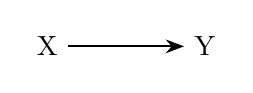
\begin{tikzpicture}[thick, >=Stealth]
        \node (x) at (-1, 0) {X};
        \node (y) at (1, 0) {Y};

        \draw[->] (x) -- (y);
    \end{tikzpicture}
    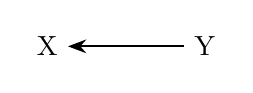
\begin{tikzpicture}[thick, >=Stealth]
        \node (x) at (-1, 0) {X};
        \node (y) at (1, 0) {Y};

        \draw[->] (y) -- (x);
    \end{tikzpicture}
    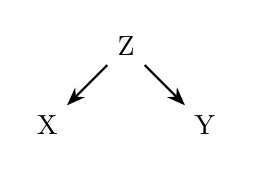
\begin{tikzpicture}[thick, >=Stealth]
        \node (x) at (-1, 0) {X};
        \node (y) at (1, 0) {Y};
        \node (z) at (0, 1) {Z};

        \draw[->] (z) -- (x);
        \draw[->] (z) -- (y);
    \end{tikzpicture}
    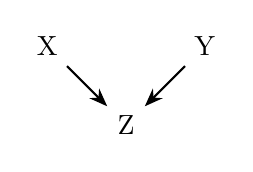
\begin{tikzpicture}[thick, >=Stealth]
        \node (x) at (-1, 0) {X};
        \node (y) at (1, 0) {Y};
        \node (z) at (0, -1) {Z};

        \draw[->] (x) -- (z);
        \draw[->] (y) -- (z);
    \end{tikzpicture}
  \end{center}
\end{frame}

\begin{frame}
  Further reading:
  \begin{itemize}
  \item Statistical Rethinking
  \item The Book of Why
  \item Causal Inference, a primer
  \end{itemize}
\end{frame}

\end{document}
